%% LaTeX Beamer presentation template (requires beamer package)
%% see http://latex-beamer.sourceforge.net/
%% idea contributed by H. Turgut Uyar
%% template based on a template by Till Tantau
%% this template is still evolving - it might differ in future releases!

\documentclass[hyperref={pdfpagelabels=false}]{beamer}

\mode<presentation>

\usepackage{graphicx}
\usetheme{isu}
\usepackage{times}
\usepackage{amsmath,amsthm, amssymb, latexsym}
\boldmath
\usepackage[english]{babel}
\usepackage[latin1]{inputenc}

\DeclareGraphicsExtensions{.pdf,.jpg,.png}
\graphicspath{{figures/}}
\usepackage{url}
\usepackage[
  natbib=true,
  backend=biber,
  uniquename=false,
  style=alphabetic,
  citestyle=authoryear
]{biblatex}
\bibliography{refs}
%\bibliographystyle{apalike}


\title[PowerGraph]{PowerGraph: Distributed Graph-Parallel Computation on Natural Graphs}
\author[David Johnston]{David Johnston}
\institute[ISU]{
    Department of Computer Science \linebreak
    Iowa State University\linebreak
    dwtj@iastate.edu
}

\date[COMS 641]{COMS 641: Data Intensive Languages and Systems - Design and Semantics}
%\date{Month X, 20XX}


% If you have a file called "university-logo-filename.xxx", where xxx
% is a graphic format that can be processed by latex or pdflatex,
% resp., then you can add a logo as follows:

%\pgfdeclareimage[height=0.25cm]{logo}{figures/logo}
%\logo{\pgfuseimage{logo}}


\begin{document}
  \begin{frame}[plain]
    \titlepage
  \end{frame}

  \section*{Overview}

\begin{frame}
\begin{itemize}
  \item The Problem
  \begin{itemize}
    \item % TODO What is the problem we solved
  \end{itemize}

  \item Our Approach
  \begin{itemize}
    \item % TODO What is our proposed solution to the problem
  \end{itemize}

  \item Evaluation
  \begin{itemize}
    \item % TODO Perhaps overview the evaluation
  \end{itemize}

  \item Benefits
  \begin{itemize}
    \item % TODO What are the benefits of our solution
  \end{itemize}
\end{itemize}
\end{frame}

  \section{The Problem}

\begin{frame}
  \frametitle{The Problem: Power Law Graphs are Common}
  \begin{itemize}
      \item An imporant class of natural graphs.
      \item A few \textit{very high-degree vertices}.
      \item Hard to partition.
      \item These vertices cause performance and scalability challenges for
            existing graph-parallel systems.
  \end{itemize}
\end{frame}

\subsection{Some Background on Power Law Graphs}

\begin{frame}
    \textbf{Q:} What's a Power Law Graph?

    \textbf{A:} A graph whose vertex degree distribution is a power law
    distribution.
\end{frame}

\begin{frame}
  \frametitle{Power Law Functions Have A Characteristic Shape}
  \begin{figure}
    \centering
    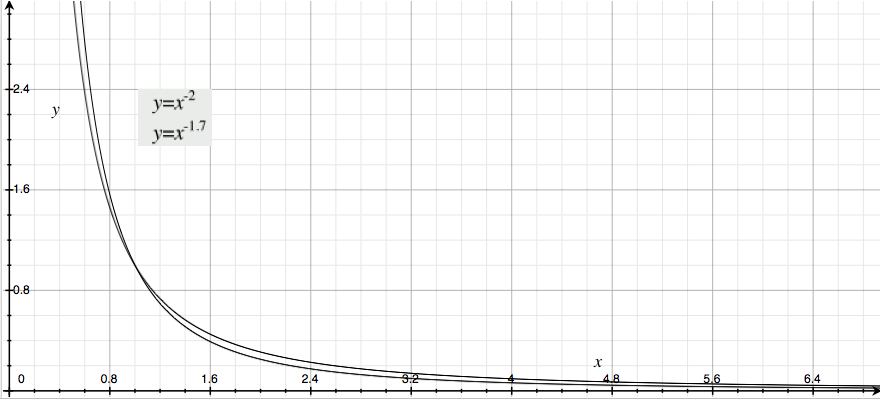
\includegraphics[scale=0.29]{two_power_law_functions}
    \caption{Two power law functions ($\alpha = 1.7$ and $\alpha = 2$) on a
             Cartesian coordinate system. A \textit{power law} is a
             proportionality relation between two values of the form
             $y \propto x^{-\alpha}$, where $\alpha$ is positive. A power law
             \textit{distribution} is just a probability distribution of this
             form.}
  \end{figure}
\end{frame}

\begin{frame}
  \frametitle{Many Natural Graphs Are Power Law Graphs}
  \begin{figure}
    \centering
    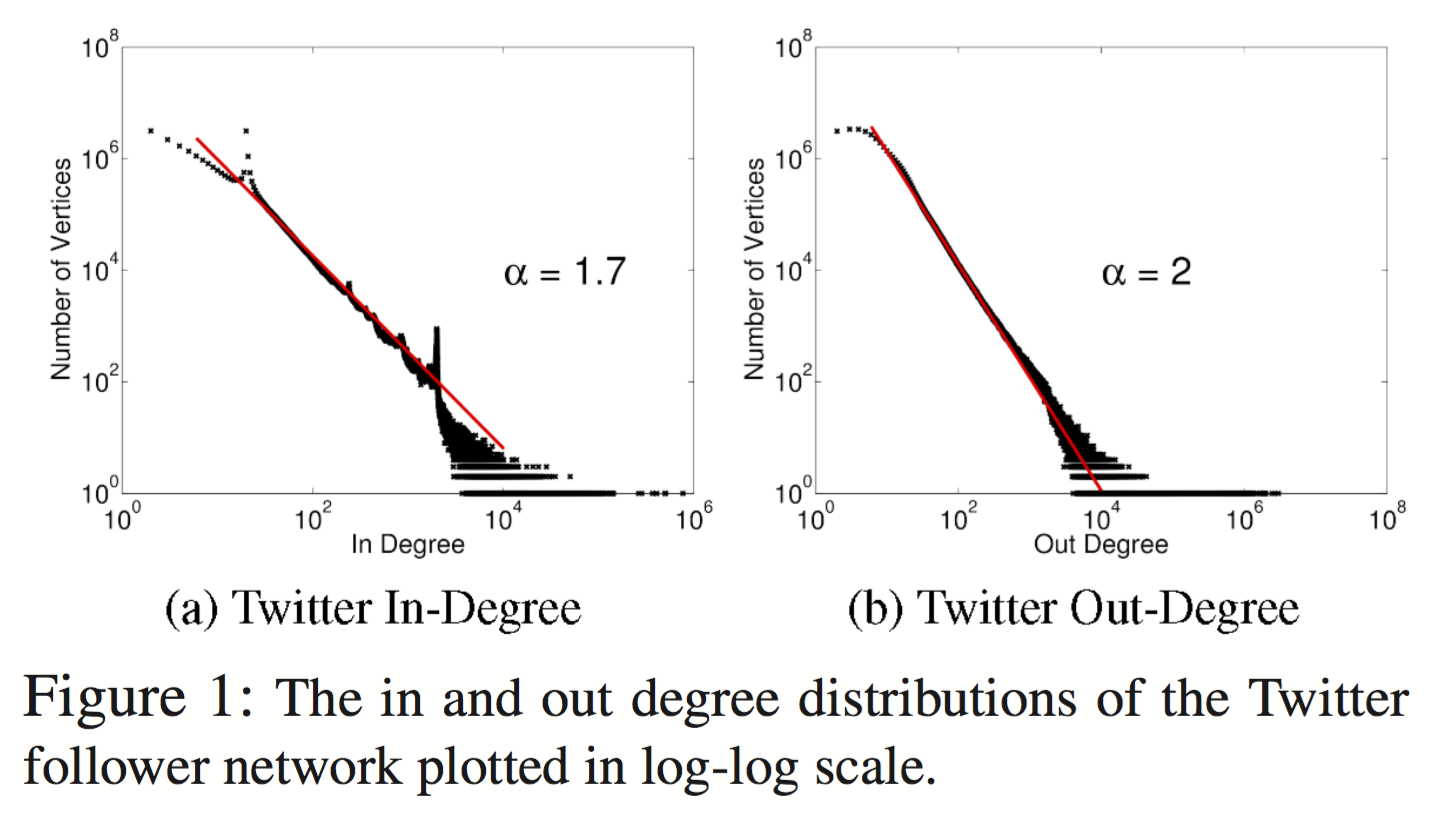
\includegraphics[scale=0.17]{gonzalez_osdi_2012_figure_1}
    \caption{\cite[OSDI '12]{gonzalez2012powergraph}}
  \end{figure}
\end{frame}

\begin{frame}
  \frametitle{A Small Number of Vertices are of Very High Degree}
  \begin{figure}
    \centering
    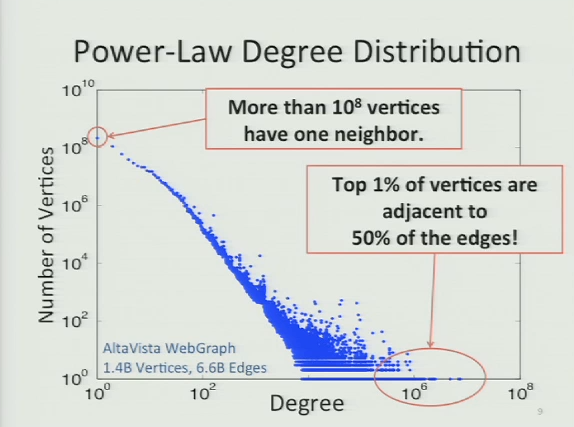
\includegraphics[scale=0.32]{gonzalez_osdi_2012_slide_9}
    \caption{\cite[OSDI '12 Slides]{gonzalez2012powergraph-slides}}
  \end{figure}
\end{frame}

\begin{frame}
  \frametitle{Power Law Graphs Are Hard to Partition}
  \begin{figure}
    \centering
    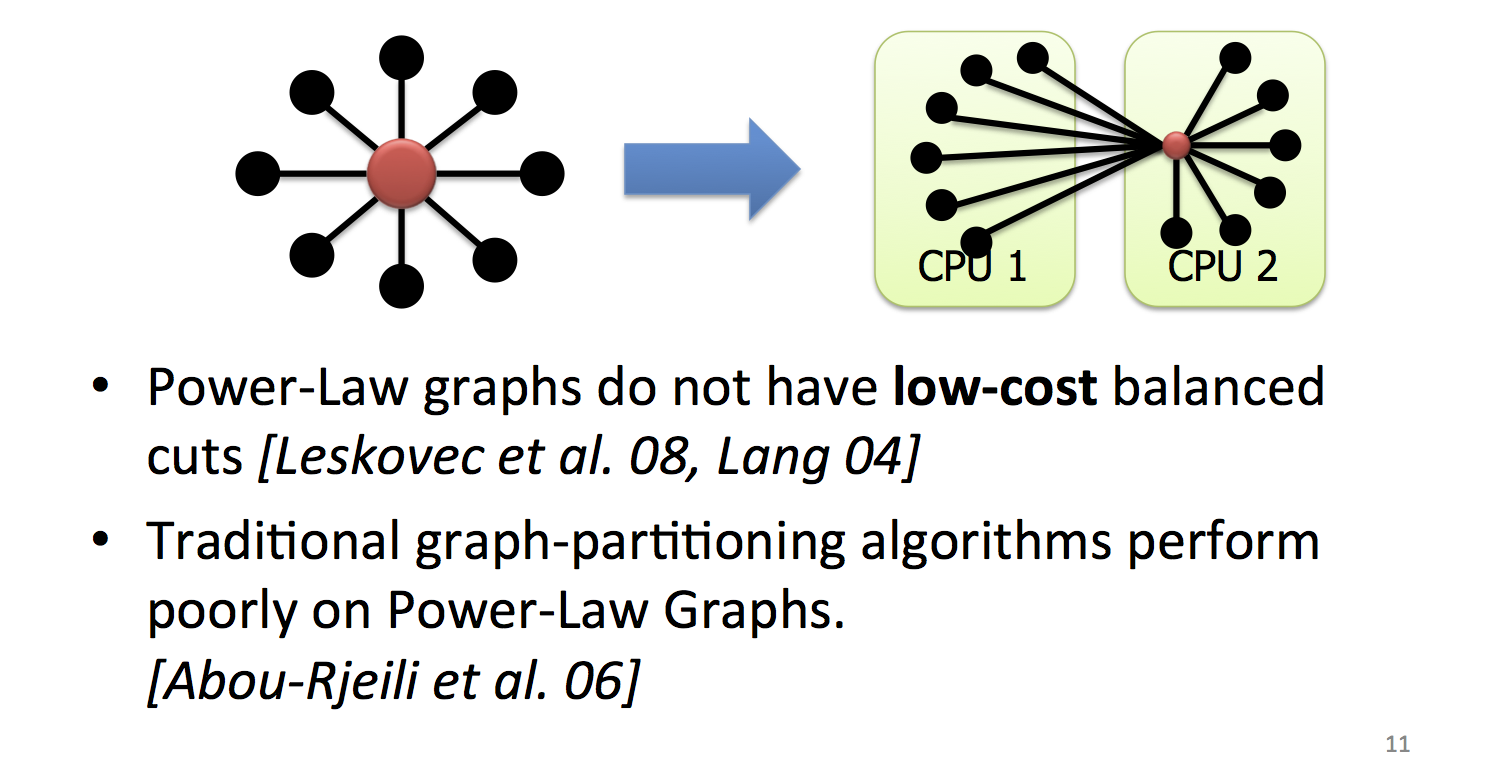
\includegraphics[scale=0.30]{gonzalez_osdi_2012_slide_11}
    \caption{\cite[OSDI '12 Slides]{gonzalez2012powergraph-slides}}
  \end{figure}
\end{frame}


\subsection{Some Background on Graph-Parallel Abstractions}

\begin{frame}
  \frametitle{Graph-Parallel Abstractions (A Review)}
  ``A graph parallel abstraction consists of a \textit{sparse} graph
  $G = \{V,E\}$ and a vertex-program $Q$ which is executed in parallel on each
  vertex $v \in V$ and can interact\ldots with neighboring
  instances.''\footnote{\cite[OSDI '12]{gonzalez2012powergraph}}


\end{frame}

\begin{frame}
  \frametitle{Graph-Parallel Abstractions (A Review)}
  ``In contrast to more general message passing models, graph-parallel
  abstractions constrain the interaction of vertex-program (sic) to a graph
  structure enabling the optimzation of data-layout and
  communication.''\footnote{\cite[OSDI '12]{gonzalez2012powergraph}}
\end{frame}

\begin{frame}
  \frametitle{Graph-Parallel Abstractions Used For Comparison}
  User-defined vertex programs run in parallel on many nodes:
  \begin{itemize}
    \item \textbf{Pregel:}\footnote{\cite[SIGMOD '10]{malewicz2010pregel}}
      \begin{itemize}
        \item Programs communicate via message passing along graph.
        \item Programs can change graph topology.
        \item Vertices own their state and state of their outgoing edges.
        \item Consistency via supersteps using a master node.
      \end{itemize}
    \item \textbf{GraphLab:}\footnote{\cite[VLDB '12]{low2012distributed}}
      \begin{itemize}
        \item Programs read/write shared data on a distributed graph.
        \item Graph topology is fixed.
        \item Good concurrency via smart scheduling of programs.
        \item Serializability via locking and inter-node messages.
      \end{itemize}
  \end{itemize}
\end{frame}


\subsection{Analysis of Previous Vertex Program Abstractions}

\begin{frame}
  \frametitle{Analysis of Previous Vertex Program Abstractions}
  \begin{itemize}
  \item The authors analyze---under the assumption of power law graphs--both
        Pregel and GraphLab.
  \item They describe some problems (e.g. work imbalance and communication
        overhead) as a consequence of edge-cuts.
  \item Only a part of this analysis is discussed here.
  \end{itemize}
\end{frame}

\begin{frame}
  \frametitle{Pregel Message Combiners Effective on Fan-In}
  \begin{figure}
    \centering
    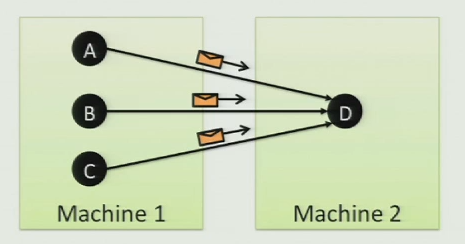
\includegraphics[scale=0.40]{gonzalez_osdi_2012_slide_22a}
    \caption{\cite[OSDI '12 Slides]{gonzalez2012powergraph-slides}}
  \end{figure}
\end{frame}

\begin{frame}
  \frametitle{Pregel Message Combiners Effective on Fan-In}
  \begin{figure}
    \centering
    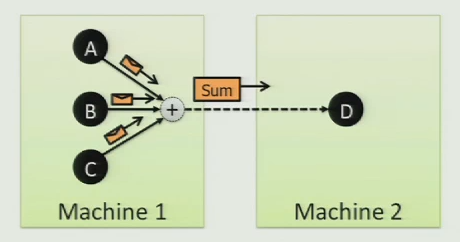
\includegraphics[scale=0.40]{gonzalez_osdi_2012_slide_22b}
    \caption{\cite[OSDI '12 Slides]{gonzalez2012powergraph-slides}}
  \end{figure}
\end{frame}

\begin{frame}
  \frametitle{Pregel Struggles with Fan-Out: Comms Overhead}
  \centering
  \large{\textit{Combiners not applicable on fan-out.}}
  \begin{figure}
    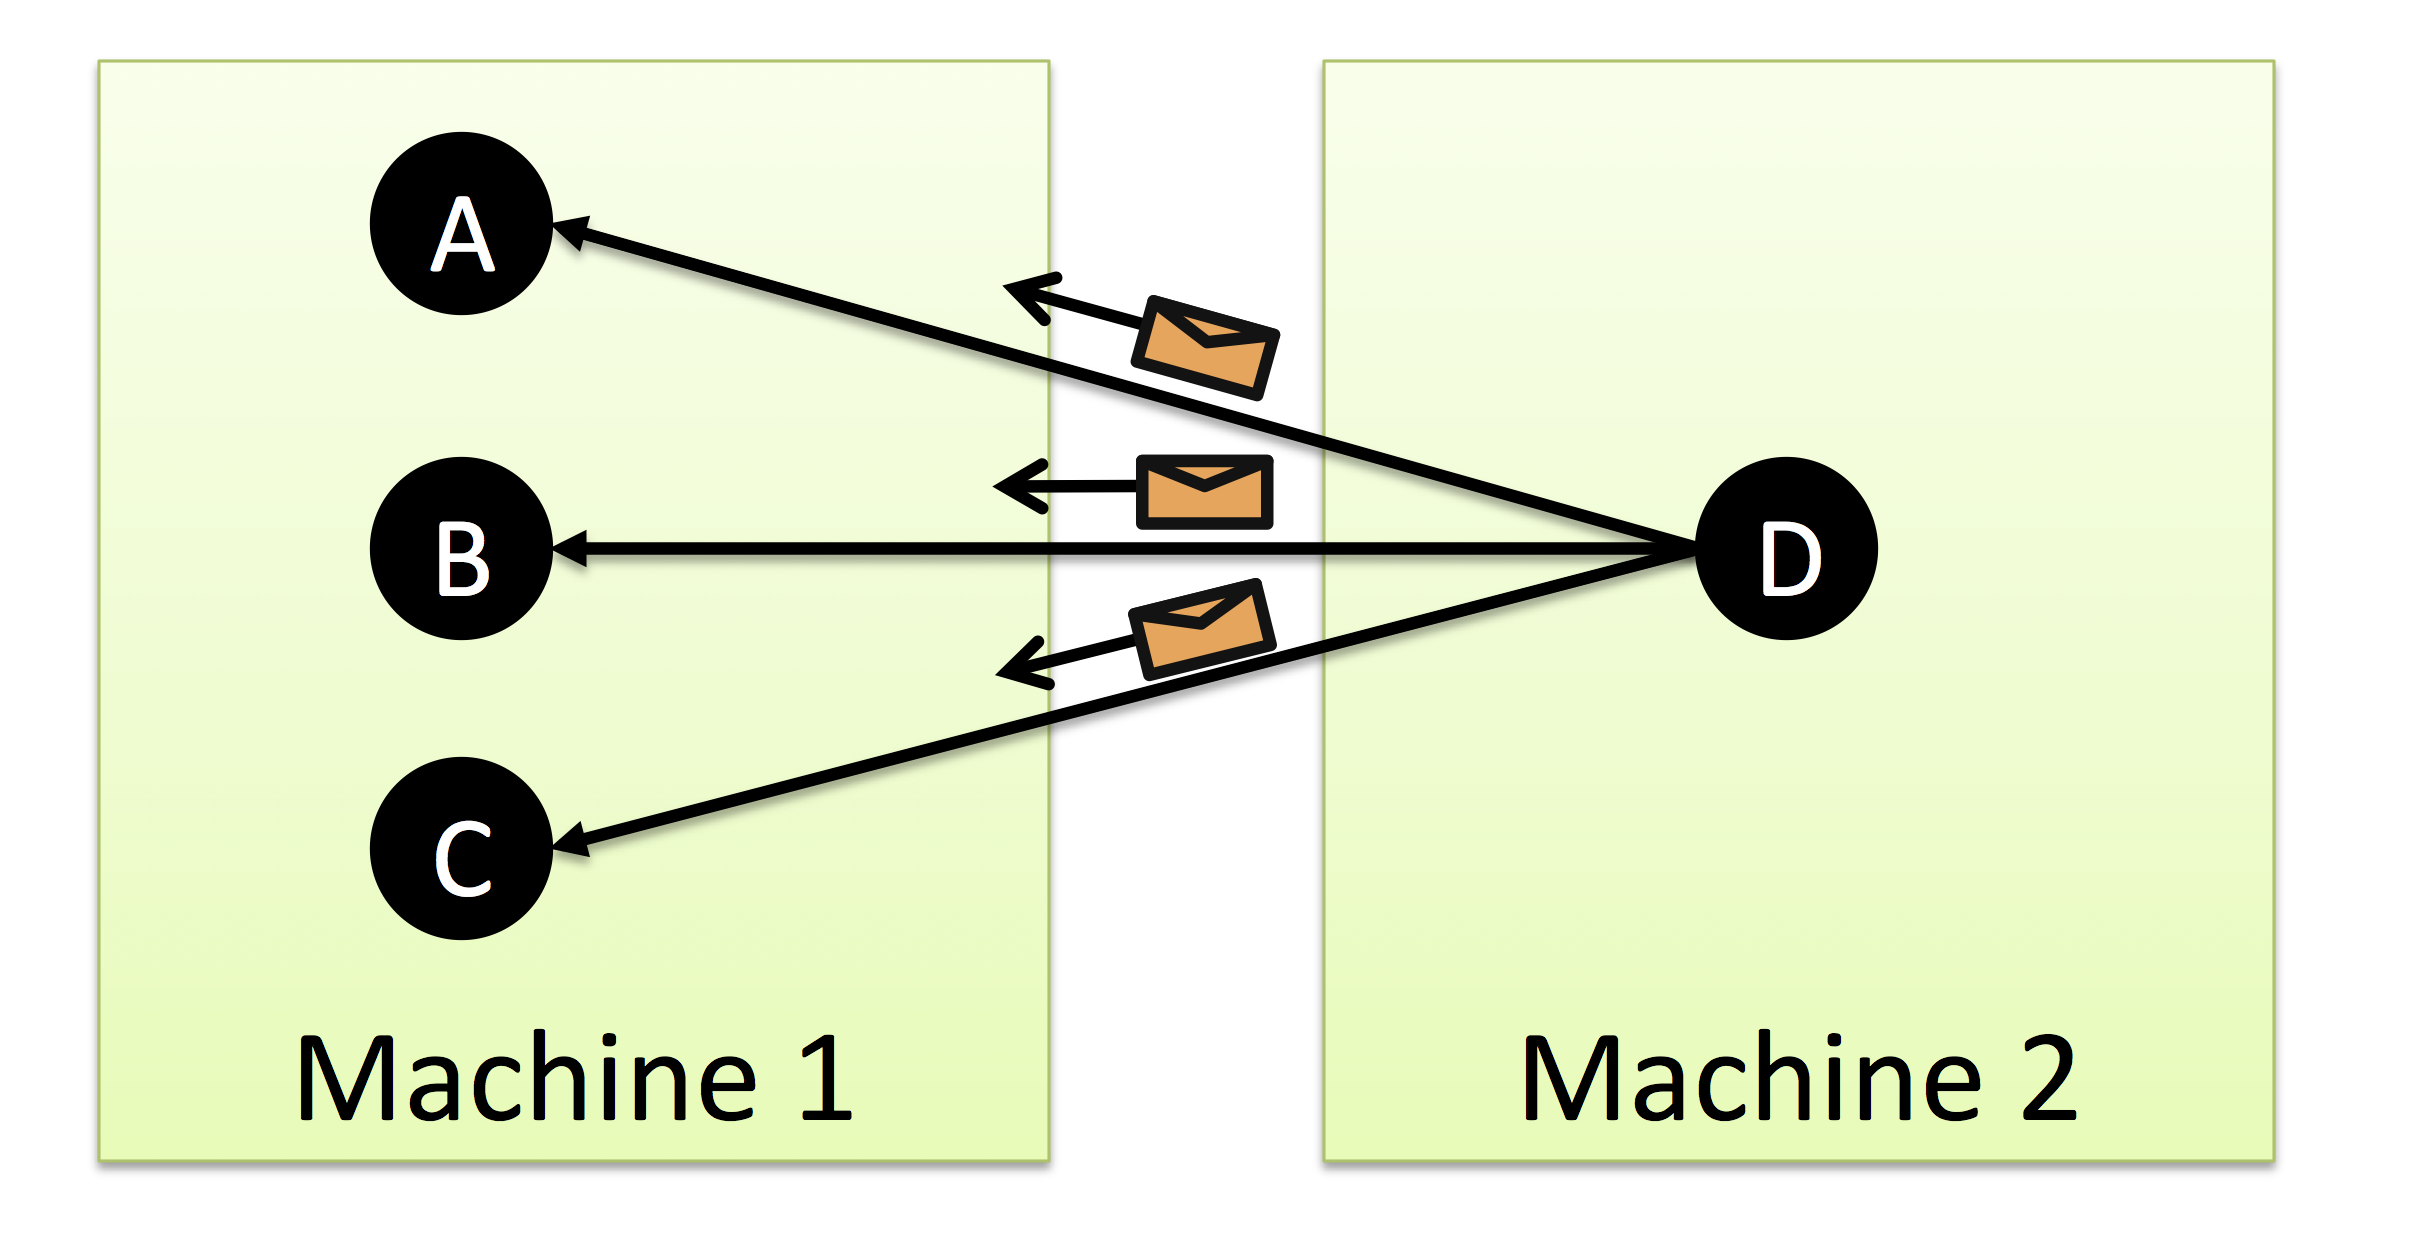
\includegraphics[width=0.6\textwidth]{gonzalez_osdi_2012_slide_23}
    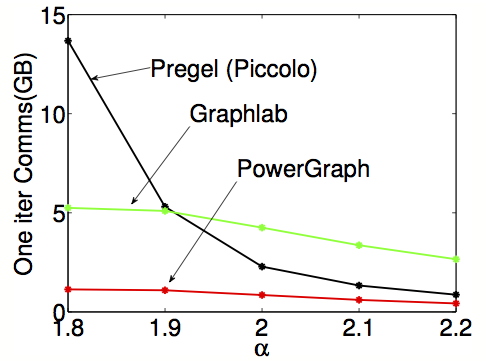
\includegraphics[width=0.4\textwidth]{gonzalez_osdi_2012_figure_9d}
    \caption{\cite[OSDI '12 Slides]{gonzalez2012powergraph-slides};
    \cite[OSDI '12]{gonzalez2012powergraph}}
  \end{figure}
\end{frame}

\begin{frame}
  \frametitle{Pregel Struggles with Fan-Out: Work Imbalance}
  \centering
  \large
  \textit{Pregel vertex program execution linear out-edge degree.}

  \begin{figure}
    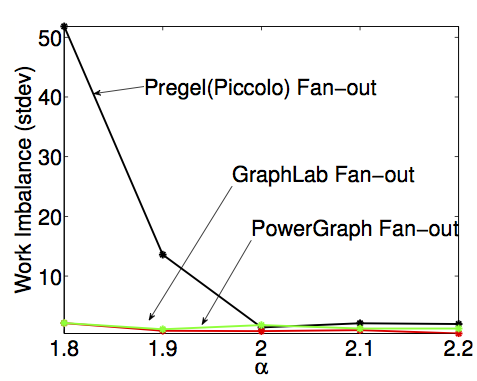
\includegraphics{gonzalez_osdi_2012_figure_9b}
    \caption{\cite[OSDI '12 Slides]{gonzalez2012powergraph-slides};
    \cite[OSDI '12]{gonzalez2012powergraph}}
  \end{figure}
\end{frame}


\subsection{The Challenges of Processing Power Law Graphs}

\begin{frame}
  \begin{figure}
    \centering
    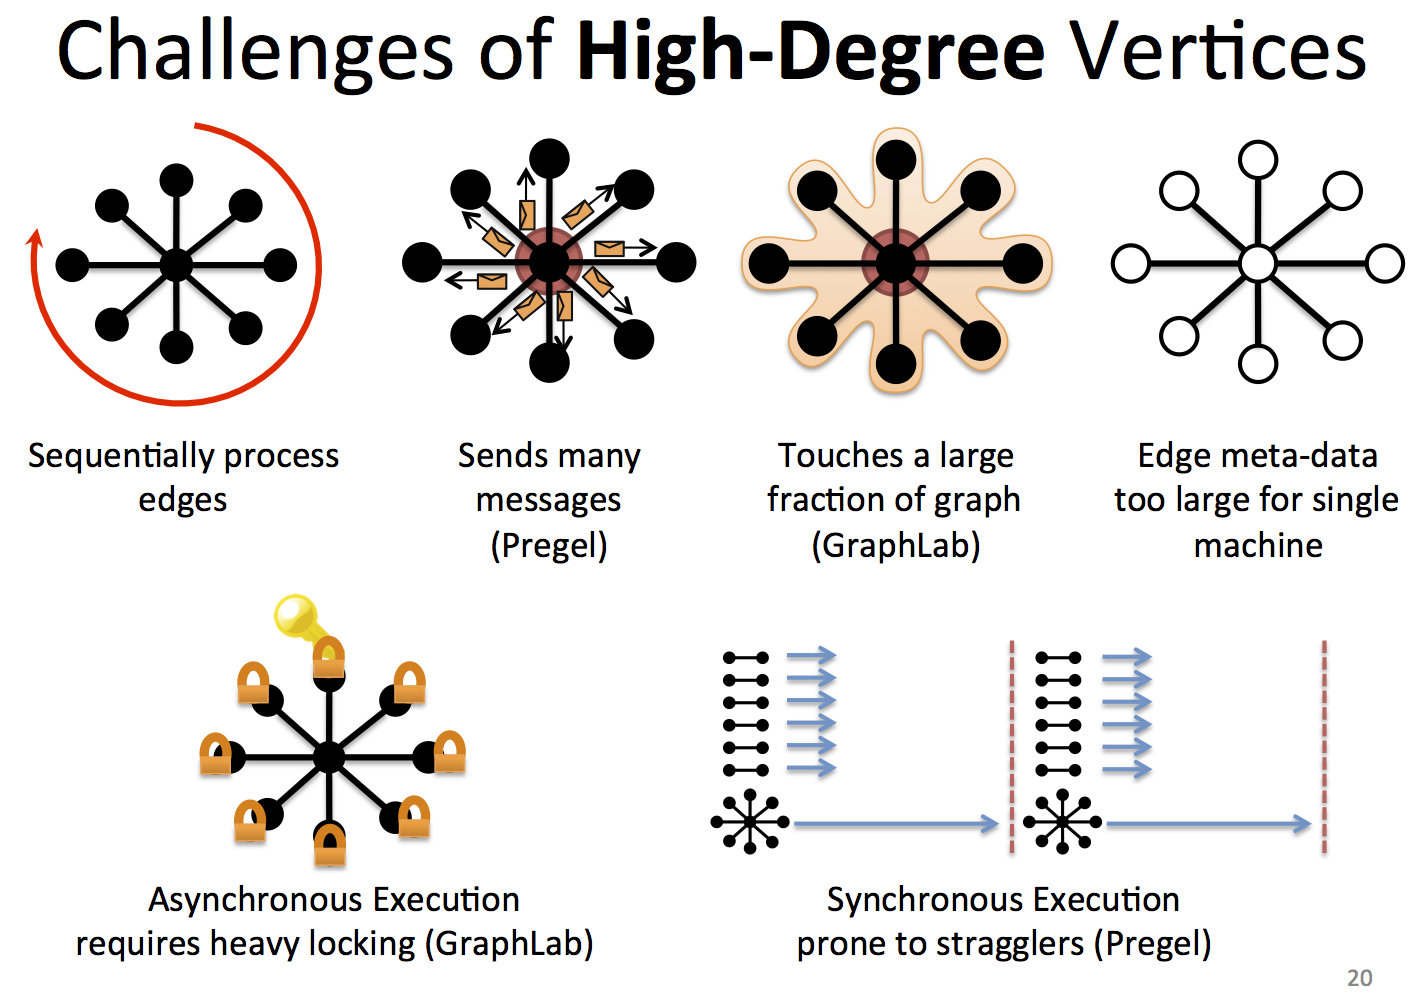
\includegraphics[scale=0.35]{gonzalez_osdi_2012_slide_20}
    \caption{\cite[OSDI '12]{gonzalez2012powergraph-slides}}
  \end{figure}
\end{frame}

\begin{frame}
  \frametitle{Challenges}
  The authors identify five ways in which these these properties of power law
  graphs create challenges for optimizations within pre-existing graph parallel
  abstractions:
  \begin{itemize}
    \item Work Balance
    \item Partitioning
    \item Communication
    \item Storage
    \item Computation
  \end{itemize}
\end{frame}

  \section{Our Approach}

\begin{frame}
\begin{itemize}
  \item % TODO What was our solution
\end{itemize}
\end{frame}

  \section{Evaluation}

\begin{frame}{Evaluation}
  \begin{itemize}
    \item \textbf{Evaluated:} Three implemented graph partitioning algorithms.
          \begin{itemize}
            \item Random
            \item Oblivious
            \item Coordinated
          \end{itemize}
    \item \textbf{Evaluated:} Three implemented PowerGraph abstraction runtimes.
          \begin{itemize}
            \item{Bulk Synchronous}
            \item{Asynchronous}
            \item{Asynchronous Serializable}
          \end{itemize}
    \item \textbf{Not Evaluated:} Performance relative to other similar
          frameworks/languages.
  \end{itemize}
\end{frame}


\subsection{Evaluating 3 Graph Partitioning Methods}

\begin{frame}
  \frametitle{\small{Do Improved V-Cut Methods Reduce Replication on Big Graph
              Datasets?}}
  \centering
  \begin{figure}
    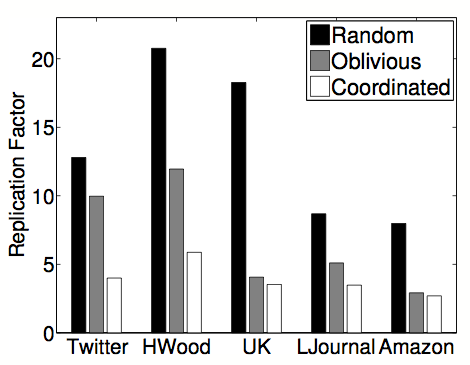
\includegraphics{gonzalez_osdi_2012_figure_7a}
    \caption{\cite[OSDI '12]{gonzalez2012powergraph}}
  \end{figure}
\end{frame}

\begin{frame}
  \frametitle{\small{Do Improved V-Cut Methods Reduce Runtime on Big Graph
              Analysis Tasks?}}
  \centering
  \begin{figure}
    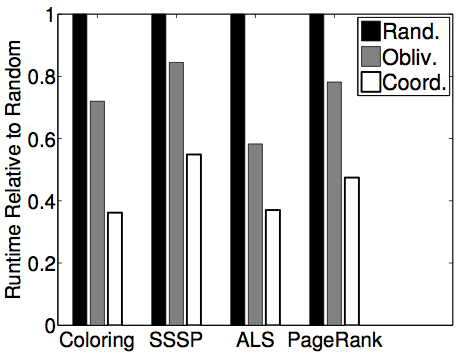
\includegraphics{gonzalez_osdi_2012_figure_7b}
    \caption{\cite[OSDI '12]{gonzalez2012powergraph}}
  \end{figure}
\end{frame}

\begin{frame}
  \frametitle{\small{Do Improved V-Cut Methods Improve Scaling of Replication
              Rates? (Twitter)}}
  \centering
  \begin{figure}
    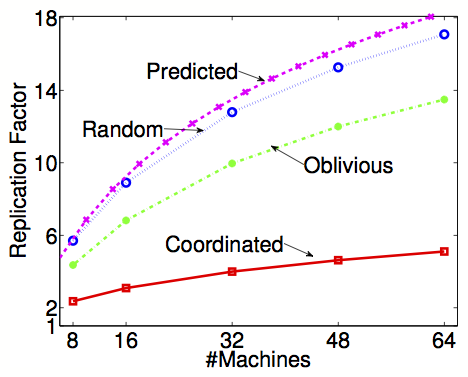
\includegraphics{gonzalez_osdi_2012_figure_8a}
    \caption{\cite[OSDI '12]{gonzalez2012powergraph}}
  \end{figure}
\end{frame}

\begin{frame}
  \frametitle{\small{Do V-Cut Algorithms \textit{Themselves} Scale Well?
              (Twitter)}}
  \centering
  \begin{figure}
    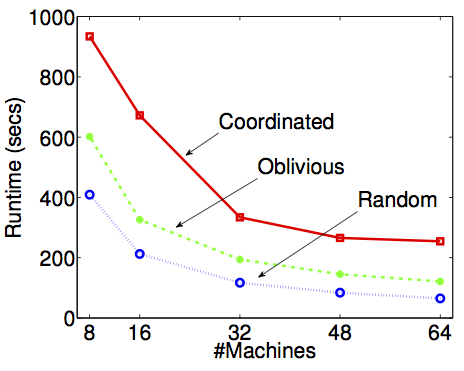
\includegraphics{gonzalez_osdi_2012_figure_8b}
    \caption{\cite[OSDI '12]{gonzalez2012powergraph}}
  \end{figure}
\end{frame}

\begin{frame}
  \textbf{TODO:} Include graphs/charts for your evaluation
\end{frame}

  \section*{Summary}

\begin{frame}{Related Work}
  \begin{itemize}
    \item \textbf{TODO:} Talk about related work here
  \end{itemize}
\end{frame}


\begin{frame}{Future Work}
  \begin{itemize}
    \item \textbf{TODO:} Talk about future work/limitations here
  \end{itemize}
\end{frame}


\begin{frame}
\begin{itemize}
  \frametitle{Overview}
  \item The Problem: Power Law Graphs are Common
  \begin{itemize}
    \item An imporant class of natural graphs.
    \item A few \textit{very high-degree vertices}.
    \item Hard to partition.
    \item These vertices cause performance and scalability challenges for
          existing graph-parallel systems.
  \end{itemize}
\end{itemize}
\end{frame}

\begin{frame}
\begin{itemize}
  \frametitle{Overview}
  \item The Approach: The PowerGraph Abstraction
  \begin{itemize}
    \item \textbf{GAS}: A new 3-phase vertex-program methodology.
    \item ``Think like a vertex.'' \citep[SIGMOD '10]{malewicz2010pregel}
    \item Graph partitioning via vertex-cut, \textit{not} edge-cut (3 variants).
    \item Three execution modes (varying guarantees).
  \end{itemize}

  \item Evaluation:
  \begin{itemize}
    \item Evaluate three V-cut graph partitioning methods.
    \item Evaluate three execution modes.
  \end{itemize}
\end{itemize}
\end{frame}

\begin{frame}
\begin{beamercolorbox}[center]{white}
  {\Large Questions?}

  \vspace{2em}\hfill

  \url{http://www.cs.iastate.edu/~dwtj}
\end{beamercolorbox}
\end{frame}


  \begin{frame}[allowframebreaks]
    \printbibliography
  \end{frame}

  \appendix

% make sure you have a blank slide in case you accidentally go past your conclusion
\begin{frame}[plain]
\end{frame}


% these slides are to help answer potential questions and generally arent shown
% unless needed or there is extra time
\begin{frame}[plain]{Hidden Slide 1}
\end{frame}

\begin{frame}[plain]{Hidden Slide 2}
\end{frame}

\end{document}
